\documentclass[../EngineeringJournal_CDavis.tex]{subfiles}

\begin{document}

%%%%%%%%%%%%%%%%%%%%%%%%%%%%%%%%%%%%%%%%%%%%%%%%%%%%%
%%%%%%%%%%%%%%%%%%%%%%%%%%%%%%%%%%%%%%%%%%%%%%%%%%%%%

\chapter[Legacy InterVlan Implementation]{Legacy InterVlan\linebreak[1]
Implementation \hspace*{\fill March 5, 2020}}
\noindent\textbf{{Packet Tracer Lab 14} \hspace*{\fill}{\textbf{CIT 167}}}\linebreak[1]
{{Spring 2020} \hspace*{\fill}{Chaz Davis}}                             
%===================================
%===================================


\hspace{0.2cm}
\begin{tcolorbox}[width=6.3in]
\scriptsize 
implement
  \begin{outline}
    \1 vlans
    \1 trunks
  \end{outline}
\end{tcolorbox}
\hspace{0.2cm}
\normalsize  
  
\clearpage

%===================================
\mysection{\textbf{Part 1: Configuring and verifying the network}}

I setup the Configuration according to the handout. I then, configured the IP
address, default gateways, and subnet masks on each of the PCs.
I Next ran the commands on R1, and then the commands on S1. I had to go back
and run {\scriptsize{\verb$int g0/1 no shut$}\normalsize} on R1.

After that I was able to successfully ping from PC1 to PC3.


\begin{figure}[!hbt]\centering
\subfloat[Pinging from PC1 to
PC3]{\label{success14ping}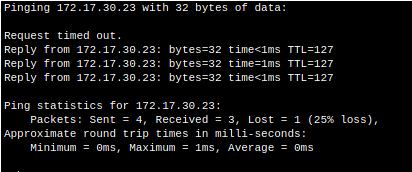
\includegraphics[width=.45\linewidth]{Figures/2020-03-08-194333_412x172_scrot.png}}\par
\subfloat[Successful network
architecture]{\label{success14arch}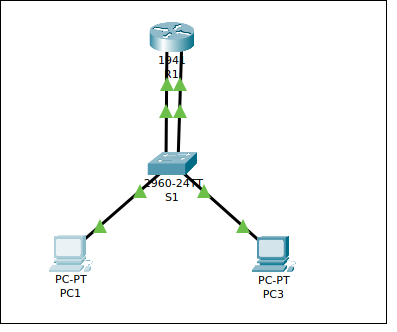
\includegraphics[width=.45\linewidth]{Figures/2020-03-08-194344_397x332_scrot.png}}\par
\caption{Successful Lab layout}
\label{success14}
\end{figure}








%===================================

\end{document}
